\documentclass[aspectratio=169,11pt]{beamer}

\usepackage{fontspec}
\setsansfont{Arial}
\setmainfont{Times New Roman}
\setmonofont{Courier New}
\usepackage{polyglossia}
\setmainlanguage{russian}
\setotherlanguage{english}
\newfontfamily\cyrillicfonttt{Courier New}

\usepackage{amsmath,amssymb,mathtools}
\usepackage{graphicx}
\usepackage{booktabs}
\usepackage{animate}
\usepackage{hyperref}
\usepackage[backend=biber,style=numeric,sorting=none]{biblatex}
\addbibresource{references.bib}

\usetheme{default}
\usecolortheme{default}
\setbeamertemplate{navigation symbols}{}
\setbeamertemplate{footline}[frame number]
\setbeamertemplate{caption}[numbered]
\graphicspath{{../assets/}}

\newcommand{\fitimage}[1]{\includegraphics[width=0.94\textwidth,height=0.72\textheight,keepaspectratio]{#1}}
\DeclareMathOperator*{\argmin}{arg\,min}

\title[Метод роя частиц]{Метод роя частиц}
\subtitle{Particle Swarm Optimization}
\author{Ластовецкий Дмитрий}
\institute{Университет ИТМО\\Институт математики}
\date{2026}

\begin{document}

\begin{frame}
    \titlepage
\end{frame}

\begin{frame}{Задача}
    \centering
    \Large
    \[
        \min_{x\in D} f(x),\qquad x\in\mathbb{R}^d
    \]
    \vspace{0.1cm}
    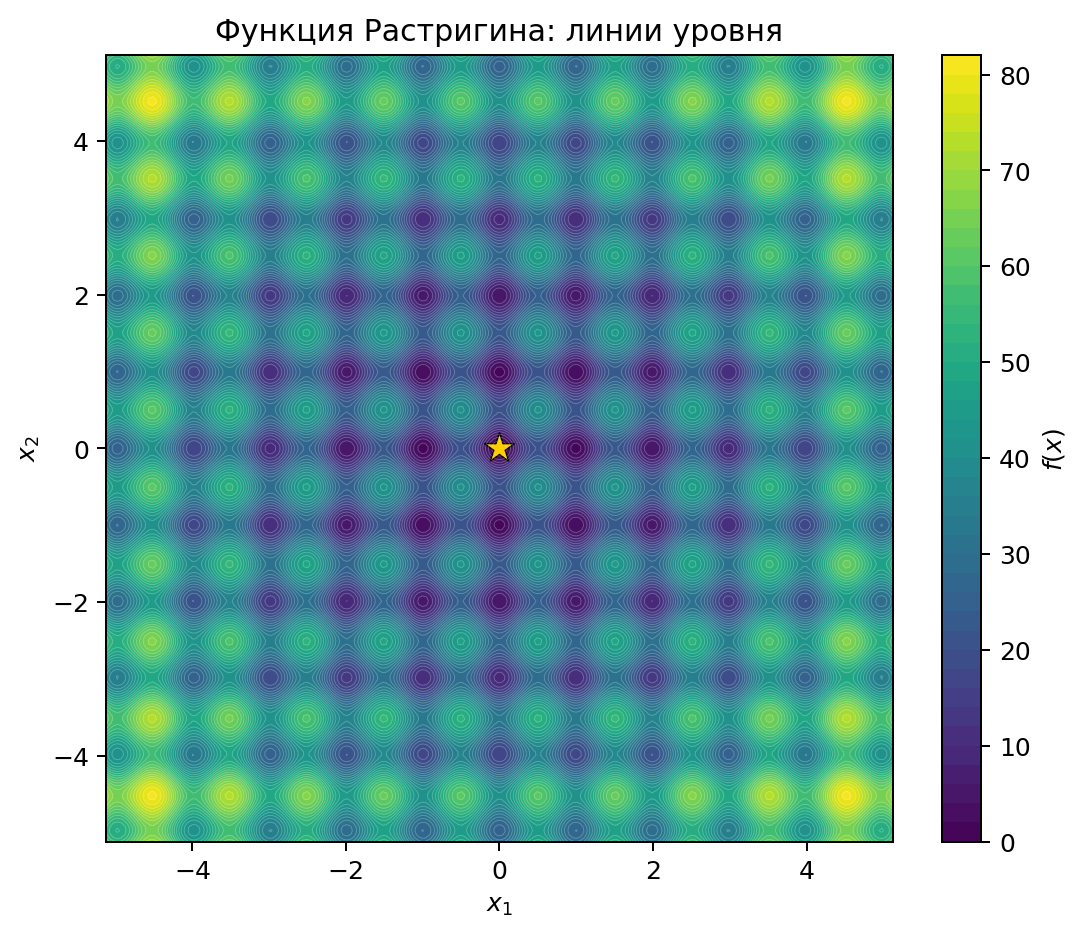
\includegraphics[width=0.74\textwidth,height=0.56\textheight,keepaspectratio]{rastrigin_contour.png}
\end{frame}

\begin{frame}{Идея PSO}
    \centering
    \fitimage{pso_step_scheme.png}
\end{frame}

\begin{frame}{Формула шага}
    \large
    \[
        v_i^{t+1}
        =
        \omega v_i^t
        + c_1 r_{1,i}^t\odot(p_i^t-x_i^t)
        + c_2 r_{2,i}^t\odot(g^t-x_i^t)
    \]
    \[
        x_i^{t+1}=\Pi_D(x_i^t+v_i^{t+1})
    \]
    \vspace{0.1cm}
    \footnotesize
    \begin{tabular}{p{0.27\textwidth}p{0.64\textwidth}}
        \(x_i^t\in\mathbb{R}^d\) & положение частицы \(i\) на итерации \(t\)\\
        \(v_i^t\in\mathbb{R}^d\) & скорость частицы\\
        \(p_i^t\) & лучшая точка, найденная самой частицей\\
        \(g^t\) & лучшая точка, найденная всем роем\\
        \(\omega\) & вес инерции: насколько сохраняется прежнее движение\\
        \(c_1,c_2\) & веса личного и коллективного притяжения\\
        \(r_{1,i}^t,r_{2,i}^t\in[0,1]^d\) & случайные векторы, координаты независимы и равномерны\\
        \(\odot\) & покоординатное умножение: \((a\odot b)_j=a_jb_j\)\\
        \(\Pi_D\) & проекция или обрезка точки обратно в допустимую область \(D\)\\
    \end{tabular}
\end{frame}

\begin{frame}{Почему это может работать}
    \large
    \begin{itemize}
        \item Лучшее найденное значение не теряется:
        \[
            f(g^{t+1})\le f(g^t).
        \]
        \item Частицы исследуют разные области поиска.
        \item Инерция дает движение, а \(p_i^t\) и \(g^t\) стягивают рой к хорошим точкам.
        \item Общей гарантии глобального минимума для невыпуклых функций нет \cite{poli2007overview}.
    \end{itemize}
\end{frame}

\begin{frame}{Что такое элитизм}
    \large
    Элитизм означает, что алгоритм не забывает лучший уже найденный результат.
    \[
        g^t\in\argmin_{p\in\{p_1^t,\ldots,p_N^t\}} f(p),
        \qquad
        f(g^{t+1})\le f(g^t).
    \]
    \normalsize
    Даже если все частицы на следующем шаге уйдут в плохие точки, сохраненная точка \(g^t\) останется кандидатом на ответ. Это полезно, но не является гарантией глобального оптимума.
\end{frame}

\begin{frame}{Строго: что гарантировано}
    \large
    \begin{itemize}
        \item Элитизм дает монотонность: \(f(g^t)\) не возрастает.
        \item Если \(f\) ограничена снизу, то \(f(g^t)\) имеет предел.
        \item Для \(\mu\)-сильно выпуклой функции:
        \[
            f(g^t)-f^\star\le\varepsilon
            \Rightarrow
            \|g^t-x^\star\|\le\sqrt{2\varepsilon/\mu}.
        \]
        \item Но это не доказывает, что стандартный PSO сам достигнет такого \(t\).
    \end{itemize}
\end{frame}

\begin{frame}{Когда есть глобальная гарантия}
    \large
    Для компактной области \(D\) и непрерывной \(f\):
    \[
        A_\varepsilon=\{x\in D:f(x)-f^\star\le\varepsilon\}.
    \]
    Если алгоритм на каждой итерации имеет независимый шанс
    \(p_\varepsilon>0\) попасть в \(A_\varepsilon\), то
    \[
        \mathbb{P}(T_\varepsilon\le T)\ge 1-(1-p_\varepsilon)^T\to 1.
    \]
    \normalsize
    Это верно для случайного поиска, рестартов и PSO с достаточно сильной мутацией. Для обычного PSO без рестартов такое условие может нарушаться.
\end{frame}

\begin{frame}{Когда гарантий нет}
    \large
    \begin{itemize}
        \item Стандартный PSO может сходиться к точке, которая не является оптимумом \cite{vandenbergh2010convergence}.
        \item Возможна стагнация даже на простых функциях типа Sphere \cite{lehre2011fht,rass2015stagnation}.
        \item Для всех возможных черных ящиков не существует универсально лучшего алгоритма \cite{wolpert1997nofree}.
        \item Поэтому в невыпуклых задачах нужны повторы, рестарты, мутация или гибрид с локальным методом.
    \end{itemize}
\end{frame}

\begin{frame}{Как мерить скорость}
    \Large
    \[
        \Delta_t=f(g^t)-f^\star
    \]
    \[
        T_\varepsilon=\min\{t:\Delta_t\le\varepsilon\}
    \]
    \[
        t_{\mathrm{run}}\quad\text{в миллисекундах}
    \]
    \normalsize
    \vspace{0.2cm}
    \(T_\varepsilon\) показывает число итераций до точности, а \(t_{\mathrm{run}}\) показывает среднее реальное время одного запуска.
\end{frame}

\begin{frame}{Алгоритм}
    \centering
    \begin{tabular}{p{0.9\textwidth}}
        \toprule
        1. Случайно расставить частицы в области поиска.\\
        2. Запомнить личные лучшие точки и лучшую точку роя.\\
        3. На каждой итерации обновлять скорости и положения.\\
        4. Если частица нашла точку лучше, обновить ее память.\\
        5. Вернуть лучшую точку, найденную роем.\\
        \bottomrule
    \end{tabular}
    \vspace{0.6cm}
    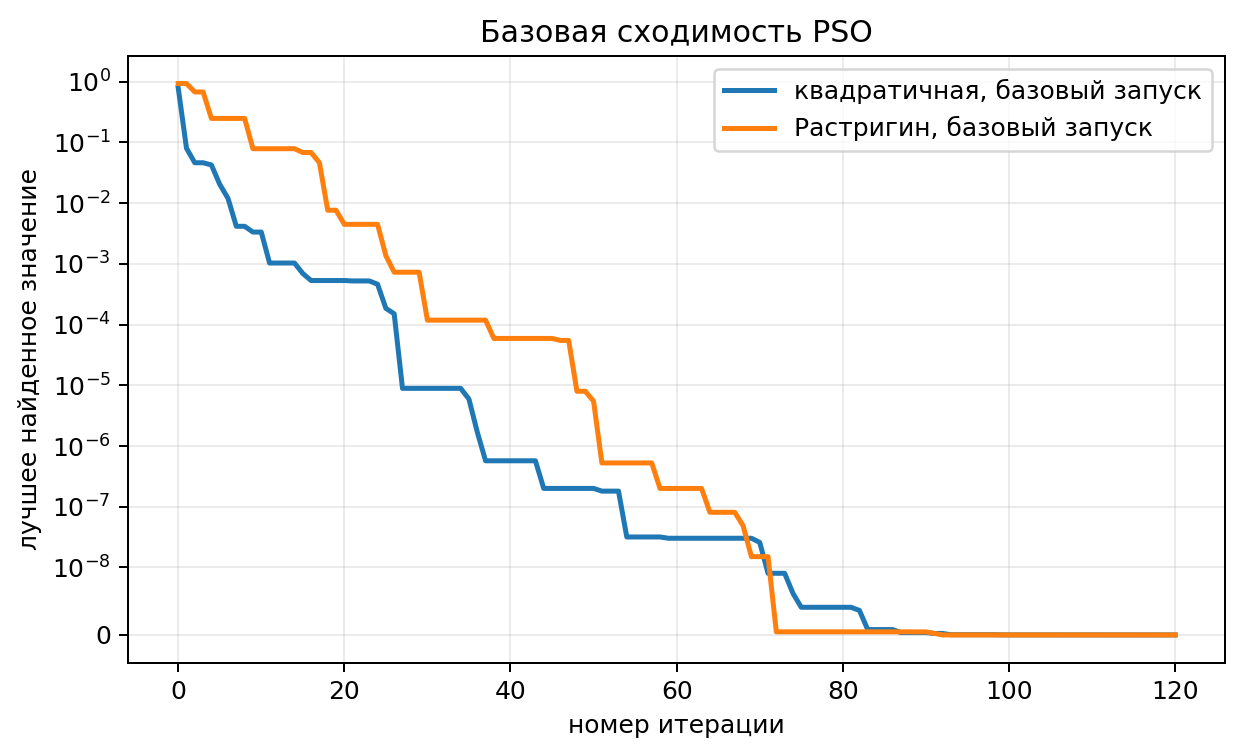
\includegraphics[width=0.7\textwidth,height=0.38\textheight,keepaspectratio]{pso_convergence.png}
\end{frame}

\begin{frame}{Сильно выпуклый пример}
    \centering
    \Large
    \[
        f_1(x)=\frac12(x_1^2+k\,x_2^2),\qquad k>0
    \]
    \[
        \nabla^2 f_1 =
        \begin{pmatrix}
            1&0\\0&k
        \end{pmatrix}
        \succeq I
    \]
    \normalsize
    Минимум единственный: \(x^\star=(0,0)\). В экспериментах \(k=10\) (базовый) и \(k=100\) (резкий рельеф).
\end{frame}

\begin{frame}{Квадратичная функция: поверхность}
    \centering
    \fitimage{quadratic_surface.png}
\end{frame}

\begin{frame}{Квадратичная функция: линии уровня}
    \centering
    \fitimage{quadratic_contour.png}
\end{frame}

\begin{frame}{Режимы на квадратичной функции}
    \large
    \begin{itemize}
        \item Базовый запуск: \(N=35\), \(\omega=0.72\), \(c_1=c_2=1.49\).
        \item Малый рой: \(N=8\), покрытие области хуже.
        \item Резкий рельеф: \(k=100\), точная доводка сложнее.
        \item Слабое притяжение: \(\omega=0.20\), \(c_1=c_2=0.35\), шаги осторожные.
    \end{itemize}
\end{frame}

\begin{frame}{Квадратичная: базовый запуск}
    \centering
    \small
    \(k=10,\; N=35,\; T=120,\; \omega=0.72,\; c_1=c_2=1.49\)

    \footnotesize базовый режим: хорошее покрытие области и сбалансированное притяжение
    \vspace{0.1cm}

    \animategraphics[autoplay,loop,width=0.82\textwidth,height=0.64\textheight,keepaspectratio]{5}{../assets/frames_quadratic/frame_}{000}{040}
\end{frame}

\begin{frame}{Квадратичная: малый рой}
    \centering
    \small
    \(k=10,\; N=8,\; T=120,\; \omega=0.72,\; c_1=c_2=1.49\)

    \footnotesize меньше частиц означает хуже начальное покрытие области поиска
    \vspace{0.1cm}

    \animategraphics[autoplay,loop,width=0.82\textwidth,height=0.64\textheight,keepaspectratio]{5}{../assets/frames_quadratic_small_swarm/frame_}{000}{040}
\end{frame}

\begin{frame}{Квадратичная: резкий рельеф}
    \centering
    \small
    \(k=100,\; N=35,\; T=120,\; \omega=0.72,\; c_1=c_2=1.49\)

    \footnotesize минимум один, но высокая обусловленность усложняет точную доводку
    \vspace{0.1cm}

    \animategraphics[autoplay,loop,width=0.82\textwidth,height=0.64\textheight,keepaspectratio]{5}{../assets/frames_quadratic_ill_conditioned/frame_}{000}{040}
\end{frame}

\begin{frame}{Квадратичная: слабое притяжение}
    \centering
    \small
    \(k=10,\; N=25,\; T=120,\; \omega=0.20,\; c_1=c_2=0.35\)

    \footnotesize движение устойчивое, но частицы делают слишком осторожные шаги
    \vspace{0.1cm}

    \animategraphics[autoplay,loop,width=0.82\textwidth,height=0.64\textheight,keepaspectratio]{5}{../assets/frames_quadratic_slow/frame_}{000}{040}
\end{frame}

\begin{frame}{Тестовая функция Растригина}
    \centering
    \Large
    \[
        f_2(x)=An+\sum_{j=1}^{n}\left(x_j^2-A\cos(2\pi x_j)\right)
    \]
    \normalsize
    \[
        x^\star=(0,\ldots,0),\qquad f_2(x^\star)=0
    \]
    \vspace{0.2cm}
    Невыпуклая benchmark-функция с большим числом локальных минимумов \cite{rastrigin1974systems,jamil2013benchmark,openturns_rastrigin}.
\end{frame}

\begin{frame}{Растригин: поверхность}
    \centering
    \fitimage{rastrigin_surface.png}
\end{frame}

\begin{frame}{Растригин: линии уровня}
    \centering
    \fitimage{rastrigin_contour.png}
\end{frame}

\begin{frame}{Режимы на функции Растригина}
    \large
    \begin{itemize}
        \item Базовый запуск: \(N=35\), стандартная широкая инициализация.
        \item Малый рой: \(N=8\), выше риск не попасть в область глобального минимума.
        \item Локальный старт около \((3,3)\): частицы видят почти только один локальный минимум.
        \item \(A=20\): рельеф становится резче, застревание в локальных минимумах сильнее.
    \end{itemize}
\end{frame}

\begin{frame}{Растригин: базовый запуск}
    \centering
    \small
    \(A=10,\; N=35,\; T=120,\; \omega=0.72,\; c_1=c_2=1.49\)

    \footnotesize широкий старт дает шанс найти область глобального минимума
    \vspace{0.1cm}

    \animategraphics[autoplay,loop,width=0.82\textwidth,height=0.64\textheight,keepaspectratio]{5}{../assets/frames_rastrigin/frame_}{000}{040}
\end{frame}

\begin{frame}{Растригин: малый рой}
    \centering
    \small
    \(A=10,\; N=8,\; T=120,\; \omega=0.72,\; c_1=c_2=1.49\)

    \footnotesize на многомодальной функции малый рой легко пропускает глобальный минимум
    \vspace{0.1cm}

    \animategraphics[autoplay,loop,width=0.82\textwidth,height=0.64\textheight,keepaspectratio]{5}{../assets/frames_rastrigin_small_swarm/frame_}{000}{040}
\end{frame}

\begin{frame}{Растригин: локальный старт}
    \centering
    \small
    \(A=10,\; N=12,\; T=120,\; \omega=0.25,\; c_1=c_2=0.55,\; x^0\approx(3,3)\)

    \footnotesize частицы видят только локальную область и почти не исследуют ноль
    \vspace{0.1cm}

    \animategraphics[autoplay,loop,width=0.82\textwidth,height=0.64\textheight,keepaspectratio]{5}{../assets/frames_rastrigin_local_start/frame_}{000}{040}
\end{frame}

\begin{frame}{Растригин: более резкий рельеф}
    \centering
    \small
    \(A=20,\; N=35,\; T=120,\; \omega=0.72,\; c_1=c_2=1.49\)

    \footnotesize локальные минимумы выражены сильнее, поэтому удачные переходы становятся реже
    \vspace{0.1cm}

    \animategraphics[autoplay,loop,width=0.82\textwidth,height=0.64\textheight,keepaspectratio]{5}{../assets/frames_rastrigin_harder/frame_}{000}{040}
\end{frame}

\begin{frame}{Сравнение сходимости}
    \centering
    \fitimage{pso_convergence.png}
\end{frame}

\begin{frame}{Разные параметры}
    \centering
    \fitimage{pso_parameter_comparison.png}
\end{frame}

\begin{frame}{Время до точности}
    \centering
    \fitimage{pso_hitting_times.png}
\end{frame}

\begin{frame}{Когда оптимум не находится}
    \large
    \begin{itemize}
        \item Малый рой плохо покрывает область поиска.
        \item Старт около локального минимума ограничивает исследование.
        \item Малые \(c_1,c_2\) и \(\omega\) дают слишком осторожные шаги.
        \item Большая амплитуда \(A\) у Растригина усиливает застревание в локальном минимуме.
    \end{itemize}
\end{frame}

\begin{frame}{Сравнение с другими методами}
    \tiny
    \begin{tabular}{p{0.19\textwidth}p{0.23\textwidth}p{0.22\textwidth}p{0.18\textwidth}}
        \toprule
        Метод & Где силен & Скорость & Успешность\\
        \midrule
        Градиентный спуск & гладкая сильно выпуклая \(f\) & линейная по итерациям & высокая, если есть градиент\\
        BFGS/Newton & гладкая локальная задача & очень быстрая около минимума & зависит от старта\\
        CMA-ES & черный ящик, плохая обусловленность & дороже PSO за итерацию & часто устойчив на DFO-бенчмарках\\
        Differential Evolution & глобальный поиск & обычно медленнее локальных методов & устойчив, но много вычислений\\
        PSO & простой параллельный глобальный поиск & быстрый ранний прогресс & чувствителен к стагнации\\
        \bottomrule
    \end{tabular}
    \vspace{0.25cm}

    По обзорам DFO нет одного победителя на всех классах задач; результаты зависят от гладкости, размерности, обусловленности и бюджета вычислений \cite{rios2013dfo,auger2010comparison}.
\end{frame}

\begin{frame}{Что важно помнить}
    \large
    \begin{itemize}
        \item PSO не требует градиента.
        \item Метод стохастический: разные запуски могут дать разные результаты.
        \item На выпуклой функции минимум один, но PSO не использует всю силу выпуклости.
        \item На Растригине популяция помогает искать глобально, но гарантий глобального минимума нет.
    \end{itemize}
\end{frame}

\begin{frame}{Код}
    \centering
    \Large
    \texttt{notebooks/pso\_demo.ipynb}
    \vspace{0.5cm}

    \normalsize
    Реализация содержит:
    \vspace{0.2cm}

    \begin{tabular}{ll}
        ядро алгоритма & \texttt{src/pso\_core.py}\\
        эксперименты & \texttt{notebooks/pso\_demo.ipynb}\\
        анимации & \texttt{scripts/generate\_assets.py}\\
    \end{tabular}
\end{frame}

\begin{frame}[allowframebreaks]{Литература}
    \tiny
    \printbibliography
\end{frame}

\end{document}
